\documentclass[german]{../spicker}

\usepackage{amsmath}
\usepackage{polynom}
\usepackage{array}   % for \newcolumntype macro
\usepackage{tikz}
\usepackage{pgfplots}
\usepackage{multirow,bigdelim}
\usepgfplotslibrary{fillbetween}

\usetikzlibrary{positioning}

\title{Lineare Algebra 2}
\author{Patrick Gustav Blaneck}
\makeindex[intoc]
\makeindex[intoc, name=Beispiele,title=Beispiele]

\newcommand{\scalarprod}[1]{\left\langle #1 \right\rangle}
\newcommand{\vektor}[1]{\begin{pmatrix*}[c] #1 \end{pmatrix*}}
\renewcommand{\span}[1]{\operatorname{span}\left(#1\right)}

\newcommand{\im}{\operatorname{im}}
\newcommand{\rg}{\operatorname{rg}}
\newcommand{\defect}{\operatorname{def}}
\newcommand{\Eig}{\operatorname{Eig}}

\renewcommand{\d}{\,\mathrm{d}}

\renewcommand{\abs}[1]{\left| #1 \right|}
\newcommand{\cis}[1]{\left( \cos\left( #1 \right) + i \sin\left( #1 \right) \right)}
\newcommand{\sgn}{\text{sgn}}
\newcommand{\diff}{\mathrm{d}}
\newcommand{\dx}{~\mathrm{d}x}
\newcommand{\du}{~\mathrm{d}u}
\newcommand{\dv}{~\mathrm{d}v}
\newcommand{\dw}{~\mathrm{d}w}
\newcommand{\dt}{~\mathrm{d}t}
\newcommand{\dn}{~\mathrm{d}n}
\newcommand{\dudx}{~\frac{\mathrm{d}u}{\mathrm{d}x}}
\newcommand{\dudn}{~\frac{\mathrm{d}u}{\mathrm{d}n}}
\newcommand{\dvdx}{~\frac{\mathrm{d}v}{\mathrm{d}x}}
\newcommand{\dwdx}{~\frac{\mathrm{d}w}{\mathrm{d}x}}
\newcommand{\dtdx}{~\frac{\mathrm{d}t}{\mathrm{d}x}}
\newcommand{\ddx}{\frac{\mathrm{d}}{\mathrm{d}x}}
\newcommand{\dFdx}{\frac{\mathrm{d}F}{\mathrm{d}x}}
\newcommand{\dfdx}{\frac{\mathrm{d}f}{\mathrm{d}x}}
\newcommand{\interval}[1]{\left[ #1 \right]}

\newcolumntype{L}{>{$}l<{$}} % math-mode version of "l" column type
\newcolumntype{R}{>{$}r<{$}} % math-mode version of "r" column type
\newcolumntype{C}{>{$}c<{$}} % math-mode version of "c" column type
\newcolumntype{P}{>{$}p<{$}} % math-mode version of "l" column type

\begin{document}
\maketitle
\tableofcontents
\newpage

%\setcounter{section}{1}

\section{Lineare Abbildungen}

\subsection{Grundlegende Eigenschaften linearer Abbildungen}

\begin{defi}{Homomorphismus}
    Eine Abbildung $f : V \to W$ heißt \emph{linear} oder ein \emph{Homomorphismus}, falls $\forall x, y \in V, \forall \lambda \in K$ gilt:
    \begin{itemize}
        \item Additivität: $f(x + y) = f(x) + f(y)$
        \item Homogenität: $f(\lambda x) = \lambda f(x)$
    \end{itemize}

    Es gilt auch:
    \begin{itemize}
        \item Für eine lineare Funktion $f$ gilt $f(0) = 0$.
        \item Die Funktion $f$ ist genau dann linear, wenn $\forall x, y \in V, \forall \lambda \in K$ gilt:
              $$
                  f(x + \lambda y) = f(x) + \lambda f(y)
              $$
        \item Summen, Vielfache linearer Abbildungen und vektorwertige Abbildungen, deren Komponenten aus linearen Abbildungen bestehen, sind wiederum linear.
    \end{itemize}
\end{defi}

\begin{defi}{Kern}
    Der \emph{Kern} einer linearen Abbildung $f : V \to W$ wird definiert durch
    $$
        \ker (f) := f^{-1}(0)
    $$

    Dabei gilt:
    \begin{itemize}
        \item $\im (f)$ ist ein Untervektorraum von $W$.
        \item $\ker (f)$ ist ein Untervektorraum von $V$.
    \end{itemize}

    Eine lineare Abbildung ist genau dann injektiv, wenn $\ker (f) = \{0\}$ gilt.
\end{defi}

\begin{bonus}{Defekt}
    Für eine lineare Funktion $f: V\to W$ definiert man den \emph{Defekt} von $f$ durch
    $$
        \defect (f) := \dim\ker (f)
    $$

    Eine lineare Abbildung ist genau dann injektiv, wenn $\defect (f) = 0$ gilt.
\end{bonus}

\begin{defi}{Rang}
    Für eine lineare Funktion $f: V\to W$ definiert man den \emph{Rang} von $f$ durch
    $$
        \rg (f) := \dim\im (f)
    $$

    Eine lineare Abbildung ist genau dann surjektiv, wenn $\rg (f) = \dim (W)$ gilt.
\end{defi}

\begin{defi}{Dimensionsformel für lineare Abbildungen (Rangsatz)}
    Es sei $f : V \to W$ linear. Dann gilt:
    $$
        \defect (f) + \rg (f) = \dim V
    $$
    bzw. äquivalent
    $$
        \dim\ker (f) + \dim\im (f) = \dim V
    $$
\end{defi}

\begin{defi}{Isomorphismus}
    Sei $f : V \to W$ linear.
    Dann ist $f$ ein \emph{Isomorphismus}, wenn $f$ bijektiv ist.

    Es gilt (für $f$ linear):
    \begin{itemize}
        \item $f$ ist genau dann ein Isomorphismus, wenn $\ker(f) = \{0\}$ und $\im(f) = W$ gilt.
        \item Gelte $\dim (V) = \dim (W)$. Dann gilt $f$ ist injektiv $\iff$ $f$ ist surjektiv $\iff$ $f$ ist bijektiv.
    \end{itemize}

    Es gilt (für $f$ Isomorphismus):
    \begin{itemize}
        \item $\dim(V) = \dim(W)$
        \item $f^{-1} : W \to V$ ist ebenfalls ein Isomorphismus.
    \end{itemize}

    Sei $\dim(V) = \dim(W) = n$, $(v_1, \ldots, v_n)$ eine Basis von $V$ und $f : V \to W$ linear.
    $f$ ist genau dann ein Isomorphismus, wenn $(f(v_1), \ldots, f(v_n))$ eine Basis von $W$ bildet.
\end{defi}

\begin{bonus}{Isomorphie}
    Seien $V$ und $W$ zwei $K$-Vektorräume
    Dann heißen $V$ und $W$ \emph{isomorph}, Schreibweise $V \simeq W$, falls ein Isomorphismus von $V$ nach $W$ existiert.

    Gilt $\dim(V) = \dim(W) = n$, dann gilt direkt $K^n \simeq V \simeq W$.
\end{bonus}

\begin{defi}{Automorphismus}
    Sei $f : V \to W$ linear.
    Dann ist $f$ ein \emph{Automorphismus}, wenn $f$ bijektiv ist und $V = W$.
\end{defi}

\begin{defi}{Endomorphismus}
    Eine lineare Abbildung $f : V \to V$ heißt \emph{Endomorphismus}.
\end{defi}

\subsection{Matrizen und lineare Abbildungen}

\begin{defi}{Abbildungsmatrix}
    Sei $f : V \to W$ linear. Dann ist die \emph{Abbildungsmatrix} $A$ bzgl. $f$ gegeben mit
    $$
        A = \vektor{f(e_1) & \ldots & f(e_n)} \ \text{mit} \ \forall x : f(x) = Ax
    $$

    Sei $(v_1, \ldots, v_n)$ eine Basis von $V$. Dann gilt:
    \begin{itemize}
        \item $\im(f) = \scalarprod{f(v_1), \ldots, f(v_n)}$
        \item $f$ ist injektiv $\iff$ $f(v_1), \ldots, f(v_n)$ sind linear unabhängig.
    \end{itemize}
\end{defi}

\begin{defi}{Darstellungsmatrix}
    Sei $f : V \to W$ linear, $\mathcal{B}_V = (v_1, \ldots, v_n)$ eine Basis von $V$ und $\mathcal{B}_W = (w_1, \ldots, w_m)$ eine Basis von $W$.
    Dann ist
    $$
        M^{\mathcal{B}_V}_{\mathcal{B}_W} (f) = \vektor{K_{\mathcal{B}_W}(f(v_1)) & \ldots & K_{\mathcal{B}_W}(f(v_1))}
    $$
    die \emph{Darstellungsmatrix} von $f$ bezüglich der Basen $\mathcal{B}_V$ und $\mathcal{B}_W$.

    $K_{\mathcal{B}_W}(f(v_i))$ bedeutet hier, dass das Bild von $v_i$ in der Basis $\mathcal{B}_W$ kodiert wird.

    Es gilt:
    \begin{itemize}
        \item Sind $\mathcal{B}_V$ und $\mathcal{B}_W$ die Standardbasen bez. $V$ und $W$, dann gilt $M^{\mathcal{B}_V}_{\mathcal{B}_W} (f) = A$.
    \end{itemize}
\end{defi}

\subsection{Abbildungsverkettung und Matrizenmultiplikation}

\begin{defi}{Eigenschaften der Abbildungsverkettung}
    Seien $U$, $V$, $W$ $K$-Vektorräume und $f : V \to W$ sowie $g : U \to V$ linear.
    Dann ist auch $f \circ g : U \to W$ linear.

    Ist $f$ ein Isomorphismus und $\dim(V) = \dim(W)$, dann gilt:
    $$
        \rg(f\circ g) = \rg(g)
    $$
\end{defi}

\begin{defi}{Eigenschaften der Matrixmultiplikation}
    Seien $A$, $B$, $C$ so, dass die nachfolgend vorkommenden Matrixmultiplikationen definiert sind.
    Dann gilt:
    \begin{itemize}
        \item $A(BC) = (AB)C$ (Assoziativgesetz)
        \item $A(B+C) = AB+AC$ und $(A+B)C = AC+BC$ (Distributivgesetz)
        \item $(AB)^T = B^TA^T$
        \item Sei $A \in K^{m\times n}$ und $E_k \in K^{k\times k}$ die $(k\times k)$-Einheitsmatrix. Dann gilt:
              $$
                  AE_n = E_mA = A
              $$
        \item Sei $A \in K^{m\times n}$ und $0_{kl} \in K^{k\times l}$ die $(k\times l)$-Nullmatrix. Dann gilt:
              $$
                  A0_{nl} = 0_{ml} \quad \text{und} \quad 0_{km}A = 0_{kn}
              $$
        \item Das Matrixprodukt ist im Allgemeinen nicht kommutativ.
        \item Seien $x, y \in K^n$. Dann gilt:
              $$
                  \scalarprod{x, y} = x^T \cdot y
              $$
    \end{itemize}
\end{defi}

\begin{defi}{Inverse einer Matrix}
    Sei $A$ eine quadratische Matrix.
    Gibt es eine Matrix $A^{-1}$ mit
    $$
        AA^{-1} = A^{-1}A = E
    $$
    so heißt $A$ \emph{invertierbar} oder auch \emph{regulär}.
    $A^{-1}$ wird als \emph{Inverse} von $A$ bezeichnet.

    Es gilt:
    \begin{itemize}
        \item Eine lineare Abbildung $f : V \to W$ ist genau dann invertierbar, wenn ihre Darstellungsmatrix invertierbar ist.
        \item Jede invertierbare Matrix ist quadratisch.
    \end{itemize}

    Seien $A, B \in K^{n\times n}$ invertierbar.
    Dann gilt:
    \begin{itemize}
        \item $AB = E \iff BA = E \iff B = A^{-1}$
        \item $AB$ ist invertierbar, und es gilt $(AB)^{-1} = B^{-1}A^{-1}$.
        \item $A^{-1}$ ist invertierbar, und es gilt $(A^{-1})^{-1} = A$.
        \item $A^T$ ist invertierbar, und es gilt $(A^T)^{-1} = (A^{-1})^T$.
        \item Für $\lambda \in K \setminus \{0\}$ ist $\lambda A$ invertierbar, und es gilt $(\lambda A)^{-1} = \frac{1}{\lambda}A^{-1}$.
    \end{itemize}
\end{defi}

\subsection{Koordinatentransformationen}

\begin{defi}{Koordinatenabbildung}
    Sei $V$ ein $K$-Vektorraum mit einer Basis $\mathcal{B} = (b_1, \ldots, b_n)$.
    Dann existiert genau ein Isomorphismus $\varphi_{\mathcal{B}} : K^n \to V$ mit $\varphi_{\mathcal{B}}(e_i) = v_i$, $1 \leq i \leq n$.

    Der Isomorphismus $\varphi_{\mathcal{B}}$ heißt \emph{Koordinatenabbildung}.
\end{defi}

\begin{defi}{Koordinaten eines Vektors}
    Sei $V$ ein $K$-Vektorraum mit einer Basis $\mathcal{B} = (b_1, \ldots, b_n)$.
    Die Abbildung $K_{\mathcal{B}}(v)$ mit
    $$
        K_{\mathcal{B}} : V \to K^n , v = \sum^n_{i=1} \lambda_ib_i \longmapsto \vektor{\lambda_1 \\ \vdots \\ \lambda_n}
    $$
    erzeugt die \emph{Koordinaten von v bezüglich der Basis} $\mathcal{B}$.

    Es gilt:
    \begin{itemize}
        \item $K_{\mathcal{B}}(v) = \varphi^{-1}_{\mathcal{B}}(v)$
    \end{itemize}
\end{defi}

\begin{defi}{Transformationsmatrix}
    Sei ein Vektorraum $V$ mit den Basen $\mathcal{A} = (a_1, \ldots, a_n)$ und $\mathcal{B} = (b_1, \ldots, b_n)$ gegeben.

    Für einen Vektor $v$ existieren die Darstellungen $K_{\mathcal{A}}(v)$ und $K_{\mathcal{B}}(v)$.
    Es gilt:

    \begin{center}
        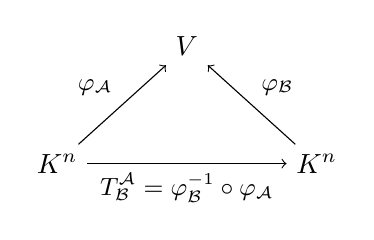
\begin{tikzpicture}
            \node (v) {$V$};
            \node [below left=of v] (k1) {$K^n$};
            \node [below right=of v] (k2) {$K^n$};

            \draw [->] (k1) -- (v) node [midway, above left] {\small $\varphi_{\mathcal{A}}$};
            \draw [->] (k2) -- (v) node [midway, above right] {\small $\varphi_{\mathcal{B}}$};
            \draw [->] (k1) -- (k2) node [midway, below] {\small $T^{\mathcal{A}}_{\mathcal{B}} = \varphi_{\mathcal{B}}^{-1} \circ \varphi_{\mathcal{A}}$};
        \end{tikzpicture}
    \end{center}


    Die Matrix $T^{\mathcal{A}}_{\mathcal{B}}$ heißt \emph{Transformationsmatrix des Basiswechsels von} $\mathcal{A}$ \emph{nach} $\mathcal{B}$

    Sei $v\in V$ beliebig, $K_{\mathcal{A}}(v) = \vektor{x_1 & \ldots & x_n}^T$ und $K_{\mathcal{B}}(v) = \vektor{y_1 & \ldots & y_n}^T$. Dann gilt:
    $$
        \vektor{y_1 \\ \vdots \\ y_n} = T^{\mathcal{A}}_{\mathcal{B}} \vektor{x_1 \\ \vdots \\ x_n}
    $$

    Sind die Koordinaten von $v$ beqüglich $\mathcal{A}$ bekannt, kann man mithilfe der Matrix $T^{\mathcal{A}}_{\mathcal{B}}$ die Koordinaten von $v$ bezüglich $\mathcal{B}$ berechnen.

    Seien $A$ und $B$ die Matrizen der Basisvektoren von $\mathcal{A}$ bzw. $\mathcal{B}$.
    Dann gilt:

    \begin{center}
        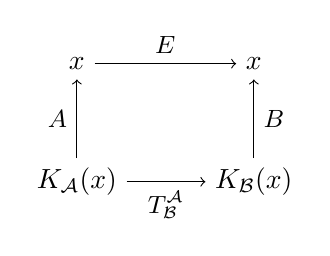
\begin{tikzpicture}
            \node (ka) {$K_{\mathcal{A}}(x)$};
            \node [right=of ka] (kb) {$K_{\mathcal{B}}(x)$};

            \node [above=of ka] (x1) {$x$};
            \node [above=of kb] (x2) {$x$};


            \draw [->] (x1) -- (x2) node [midway, above] {\small $E$};
            \draw [->] (ka) -- (x1) node [midway, left] {\small $A$};
            \draw [->] (kb) -- (x2) node [midway, right] {\small $B$};
            \draw [->] (ka) -- (kb) node [midway, below] {\small $T^{\mathcal{A}}_{\mathcal{B}}$};
        \end{tikzpicture}
    \end{center}

    Man erkennt:
    $$
        T^{\mathcal{A}}_{\mathcal{B}} = B^{-1}A
    $$
\end{defi}

\begin{defi}{Darstellungsmatrix mit Basistransformation}
    Seien $V$ und $W$ endlich erzeugt mit Basen $\mathcal{A}$ und $\mathcal{A}'$ bzw. $\mathcal{B}$ und $\mathcal{B}'$.
    Sei weiter $f : V \to W$ linear.
    Dann gilt:
    $$
        M^{\mathcal{A}'}_{\mathcal{\mathcal{B}'}}(f) = T^{\mathcal{B}}_{\mathcal{B}'} \cdot M^{\mathcal{A}}_{\mathcal{\mathcal{B}}}(f) \cdot T^{\mathcal{A}'}_{\mathcal{A}}
    $$

    Zur Visualisierung dient folgendes kommutative Diagramm:
    \begin{center}
        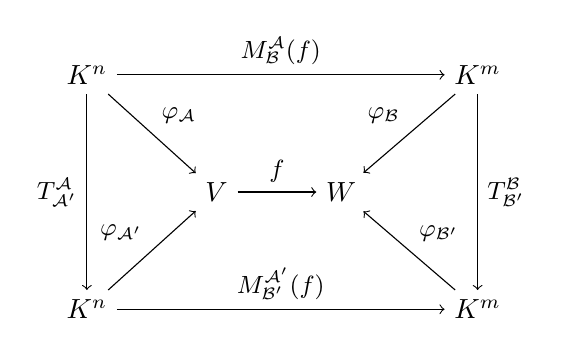
\begin{tikzpicture}
            \node (kn1) {$K^n$};
            \node [above right=of kn1] (v) {$V$};
            \node [above left=of v] (kn2) {$K^n$};
            \node [right=of v] (w) {$W$};
            \node [above right=of w] (km2) {$K^m$};
            \node [below right=of w] (km1) {$K^m$};

            \draw [->] (kn1) -- (v) node [midway, above left] {\small $\varphi_{\mathcal{A}'}$};
            \draw [->] (kn2) -- (v) node [midway, above right] {\small $\varphi_{\mathcal{A}}$};
            \draw [->] (km1) -- (w) node [midway, above right] {\small $\varphi_{\mathcal{B}'}$};
            \draw [->] (km2) -- (w) node [midway, above left] {\small $\varphi_{\mathcal{B}}$};

            \draw [->] (v) -- (w) node [midway, above] {\small $f$};

            \draw [->] (kn2) -- (km2) node [midway, above] {\small $M^{\mathcal{A}}_{\mathcal{B}} (f)$};
            \draw [->] (kn1) -- (km1) node [midway, above] {\small $M^{\mathcal{A}'}_{\mathcal{B}'} (f)$};

            \draw [->] (kn2) -- (kn1) node [midway, left] {\small $T^{\mathcal{A}}_{\mathcal{A}'}$};
            \draw [->] (km2) -- (km1) node [midway, right] {\small $T^{\mathcal{B}}_{\mathcal{B}'}$};
        \end{tikzpicture}
    \end{center}
\end{defi}

\section{Determinanten}

\begin{defi}{Elementarmatrix}
    Seien $1\leq i$, $j \leq n$ mit $i \neq j$ und $\lambda \in K \setminus \{0\}$ gegeben.
    Dann sei
    $$
        C1 := \vektor{1 & & & & \\ & \ddots & & & \\ & \lambda & \ddots & & \\ & & & \ddots & & \\ & & & & \ddots & \\ & & & & & 1} \in K^{n \times n}
    $$
    wobei der $(i, j)$-te Eintrag den Wert $\lambda$ annehmen soll und alle anderen Einträge außerhalb der Hauptdiagonalen $0$ sein sollen.

    Sei $C2$ die Matrix, die man aus der Einheitsmatrix gewinnt, indem man die $i$-te und $j$-te Spalte vertauscht, also
    $$
        C2 := \vektor{1 & & & & \\ & \ddots & & & \\ &  & 0 & &1 \\ & & & \ddots & & \\ & & 1 & & 0 & \\ & & & & & 1} \in K^{n \times n}
    $$

    Zuletzt definieren wir
    $$
        C3 := \vektor{1 & & & & \\ & \ddots & & & \\ &  & \lambda & & \\ & & & \ddots & & \\ & & & & \ddots & \\ & & & & & 1} \in K^{n \times n}
    $$

    Matrizen der Gestalt $C1$, $C2$ oder $C3$ nennt man \emph{Elementarmatrizen}.

    Es gilt:
    \begin{itemize}
        \item Die Multiplikation einer Matrix $A$ von links mit einer Elementarmatrix entspricht der Anwendung einer elementaren Zeilenoperation des Gauß-Verfahrens auf $A$.
              \subitem Notation: $Zi$ statt $Ci$
        \item Die Multiplikation einer Matrix $A$ von rechts mit einer Elementarmatrix entspricht der Anwendung einer elementaren Spaltenoperation auf $A$.
              \subitem Notation: $Si$ statt $Ci$
    \end{itemize}

    \begin{itemize}
        \item $C1$ entspricht dem Addieren von $\lambda$-mal Spalte bzw. Zeile $j$ auf Spalte bzw. Zeile $i$.
        \item $C2$ entspricht dem Tauschen von Spalte bzw. Zeile $i$ mit Spalte bzw. Zeile $j$.
        \item $C3$ entspricht dem Multiplizieren von Spalte bzw. Zeile $i$ mit $\lambda$.
    \end{itemize}
\end{defi}

\begin{defi}{Eigenschaften der Determinante}
    Für $A, B \in K^{n\times n}$ gilt:
    \begin{itemize}
        \item $S1$ und $Z1$ ändern die Determinante einer Matrix nicht. ($\det(C1) = 1$)
        \item $S2$ und $Z2$ kehren das Vorzeichen der Determinante um. ($\det(C2) = -1$)
        \item $S3$ und $Z3$ vervielfachen den Wert der Determinante um den Faktor $\lambda$. ($\det(C3) = \lambda$)
    \end{itemize}

    \begin{itemize}
        \item $\det(A) = \det(A^T)$
        \item Besitzt $A$ zwei gleiche Spalten bzw. Zeilen, so gilt $\det(A) = 0$.
        \item $A$ invertierbar $\iff \det(A) \neq 0$
        \item $\det(AB) = \det(A)\det(B)$
        \item $A$ invertierbar $\implies \det(A^{-1}) = (\det(A))^{-1}$
    \end{itemize}
\end{defi}

\subsection{Verfahren zur Berechnung der Determinante}

\begin{defi}{Laplacescher Entwicklungssatz}
    Für $A \in K^{n\times n}$ bezeichne $A_{ij}$ die Matrix in $K^{(n-1)\times (n-1)}$, die durch Streichen der $i$-ten Zeile und der $j$-ten Spalte aus $A$ hervorgeht.

    Es sei $A = (a_{ij}) \in K^{n\times n}$ und $j$ mit $1 \leq j \leq n$.
    Dann gilt:
    $$
        \det(A) = \sum^n_{i=1} (-1)^{i+j} a_{ij}\det(A_{ij})
    $$
    Man spricht von der \emph{Entwicklung der Determinante nach der j-ten Spalte}.
    Ebenso ist eine \emph{Entwicklung der Determinante nach der i-ten Zeile} möglich:
    $$
        \det(A) = \sum^n_{j=1} (-1)^{i+j} a_{ij}\det(A_{ij})
    $$
\end{defi}

\begin{defi}{Determinante mit Gauß-Algorithmus}
    Zur Berechnung mit dem Gauß-Algorithmus bringt man die gegebene Matrix $A$ mittels äquivalenter Zeilen- oder Spaltenumformungen $Z1$-$Z3$ bzw. $S1$-$S3$ auf Stufenform $B$ und errechnet dann nach Folgerung $\det(A)$ leicht als Produkt der Hauptdiagonalelelemente von $B$, multipliziert mit den Determinanten der genutzten Elementarmatrizen.
\end{defi}

\begin{bonus}{Tipps zur Determinantenberechnung}
    \begin{enumerate}
        \item Für $(2\times 2)$- und $(3\times 3)$-Matrizen empfiehlt sich die Sarrus-Regel.\footnote{Siehe Lineare Algebra 1}
        \item Die Laplace-Entwicklung ist dann vorzuziehen, wenn in einer Spalte oder Zeile nur wenige Nicht-Null-Einträge vorhanden sind, weil bei einer Entwicklung nach dieser Zeile bzw. Spalte die meisten Summanden erst gar nicht berechnet werden müssen.
        \item Es können zur Berechnung der Determinanten mehrere Verfahren kombiniert werden, z.B. $(4\times 4)$-Matrizen zuerst nach Laplace entwickeln und die dann entstehenden Determinanten von $(3\times 3)$-Matrizen direkt mit der Sarrus-Regel berechnen.
    \end{enumerate}
\end{bonus}

\begin{bonus}{Inverse einer $(2\times 2)$-Matrix}
    Sei $A$ definiert als $A = \vektor{a & b \\ c & d}$. Dann gilt:
    $$
        A^{-1} = \frac{1}{\det(A)} \vektor{d & -b \\ -c & a} = \frac{1}{ad - bc} \vektor{d & -b \\ -c & a}
    $$
\end{bonus}

\section{Lineare Gleichungssysteme}

\subsection{Lösbarkeit eines linearen Gleichungssystems}

\begin{defi}{Lineares Gleichungssystem}
    Seien $A = (a_{ij}) \in K^{m\times n}$ und $b = \vektor{b_1 & \ldots & b_m}^T$.
    Dann heißt
    $$
        \begin{aligned}
             & a_{11}x_1 &  & + \ \ldots \ + &  & a_{1n}x_n &  & = &  & b_1 \\
             & \ldots                                                       \\
             & a_{m1}x_1 &  & + \ \ldots \ + &  & a_{mn}x_n &  & = &  & b_m
        \end{aligned}
    $$
    \emph{lineares Gleichungssystem} bzgl. $(x_1, \ldots, x_n)$ mit Koeffizienten $a_{ij}$ in $K$.
    Hierbei sind $x_1, \ldots, x_n$ die \emph{Unbekannten} des Systems.

    Für $b = 0_{m1}$ nennt man das lineare Gleichungssystem \emph{homogen}, sonst \emph{inhomogen}.

    Jedes lineare Gleichungssystem kann in der Form $Ax = b$ geschrieben werden.
\end{defi}

\begin{defi}{Lösungsmenge}
    Die \emph{Lösungsmenge} $L(A, b)$ des zu $(A, b)$ gehörigen Gleichungssystems ist festgelegt durch
    $$
        L(A, b) := \{x \in K^n \mid Ax = b\}
    $$
\end{defi}

\begin{defi}{Spaltenrang}
    Die lineare Abbildung $L_A : K^n \to K^m$ sei gegeben durch $L_A(x) := Ax$. Dann sei $\rg(A) := \rg(L_A)$.
    Der \emph{Spaltenrang} $\rg_S(A)$ sei die maximale Anzahl linear unabhängiger Spaltenvektoren von $A$.

    Es gilt $\rg(A) = \rg_S(A)$.
\end{defi}

\begin{defi}{Zeilenrang}
    Für $A \in K^{m\times n}$ sei die maximale Anzahl linear unabhängiger Zeilenvektoren von $A$ der \emph{Zeilenrang} $\rg_Z(A)$ von $A$.

    Es gilt:
    $$
        \rg(A) = \rg_S(A) = \rg_Z(A)
    $$
\end{defi}

\begin{defi}{Lösbarkeit von linearen Gleichungssystemen}
    Das lineare Gleichungssystem $Ax = b$ ist genau dann lösbar, wenn gilt:
    $$
        \rg(a_1, \ldots, a_n) = \rg(a_1, \ldots, a_n, b)
    $$
    Kürzer schreibt man $\rg(A) = \rg(A, b)$.

    $Ax = b$ ist also genau dann eindeutig lösbar, falls $\ker(A) = \{0\} \iff \rg(A) = \rg(A, b) = n$.
\end{defi}

\begin{bonus}{Äquivalente Bedingungen für eindeutige Lösbarkeit}
    Sei $K \in \{\R, \C\}$.
    Für $A \in K^{n\times n}$ und die dadurch gegebene lineare Abbildung $L_A$ sind folgende Bedingungen äquivalent:
    \begin{enumerate}
        \item $A$ ist invertierbar.
        \item $Ax = 0$ hat nur die triviale Lösung $x=0$.
        \item Durch Zeilen- und Spaltenumformungen kann $A$ auf die Einheitsmatrix transformiert werden.
        \item $A$ ist darstellbar als Produkt von Elementarmatrizen.
        \item $Ax = b$ besitzt für jedes $b \in K^n$ mindestens eine Lösung.
        \item $Ax = b$ hat genau eine Lösung für jedes $b \in K^n$.
        \item $\det(A) \neq 0$
        \item $\im(A) = K^n$
        \item $L_A$ ist bijektiv.
        \item Die Spaltenvektoren von $A$ sind linear unabhängig.
        \item Die Zeilenvektoren von $A$ sind linear unabhängig.
        \item Die Spaltenvektoren von $A$ bilden eine Basis von $K^n$.
        \item Die Zeilenvektoren von $A$ bilden eine Basis von $K^n$.
        \item $\rg(A)=n$
        \item $\ker(L_A) = \{0\}$
        \item $(\ker(L_A))^\perp = K^n$
        \item Das orthogonale Komplement des von den Zeilen von $A$ aufgespannten Raums ist $\{0\}$.
        \item $A^TA$ ist invertierbar.
    \end{enumerate}
\end{bonus}

\begin{defi}{Allgemeine Lösung eines linearen Gleichungssystems}
    Sei $x_s \in K^n$ eine (spezielle) Lösung von $Ax = b$.
    Dann gilt:
    $$
        L(A, b) = x_s + \ker(A) = \{x_s + x \mid x \in \ker(A)\}
    $$
    bzw., wenn $(v_1, \ldots, v_r)$ eine Basis von $\ker(A)$ ist:
    $$
        L(A, b) = \{x + \lambda_1 v_1 + \ldots + \lambda_rv_r \mid \lambda_i \in K\}
    $$
\end{defi}

\begin{defi}{Cramersche Regel}
    Es seien $A = \vektor{a_1 & \ldots & a_n} \in K^{n\times n}$ und $x, b \in K^n$ sowie $Ax=b$ ein lineares Gleichungssystem, und es gelte $\det(A) \neq 0$.
    Seien
    $$
        A_i := \vektor{a_1 & \ldots & a_{i-1} & b & a_{i+1} & \ldots & a_n}, 1 \leq i \leq n
    $$
    Dann gilt:
    $$
        x_i = \frac{\det(A_i)}{\det(A)}, 1 \leq i \leq n
    $$
\end{defi}

\subsection{Über- und unterbestimmte lineare Gleichungssysteme}

\begin{defi}{Normalgleichung}
    Sei $p_A(b)$ die Projektion eines Vektors $b \in \R^m$ auf den von den Vektoren $A = \vektor{a_1 & \ldots & a_n} \in \R^{m\times n}$ aufgespannten Unterraum $U$, also das Bild von $A$.

    Damit existiert ein $x \in \R^n$ mit
    $$
        p_A(b) = \sum^n_{k=1} x_ka_k = Ax
    $$
    Dann gilt
    $$
        b - p_A(b) \iff \ldots \iff A^TAx = A^Tb
    $$

    Die Gleichungen $A^TAx = A^Tb$ heißen \emph{Normalgleichungen}.

    Die Normalgleichungen sind für jede relle Matrix $A \in \R^{m\times n}$ lösbar.

\end{defi}

\begin{defi}{Verallgemeinerte Inverse}
    Gegeben ist ein lineares Gleichungssystem $Ax=b$ mit $A \in \R^{m\times n}$, $x \in \R^n$, $b \in \R^m$.

    Im Fall $\rg(A) = n$ (voller Spaltenrang) existiert mit
    $$
        x = (A^TA)^{-1}A^Tb
    $$
    eine eindeutige Lösung.
    In diesem Fall heißt $(A^TA)^{-1}A^T$ \emph{verallgemeinerte Inverse} von $A$.

    Im Fall $\rg(A) = m$ (voller Zeilenrang) existiert mit
    $$
        x = A^T(AA^T)^{-1}b
    $$
    eine eindeutige Lösung.
    In diesem Fall heißt $A^T(AA^T)^{-1}$ \emph{verallgemeinerte Inverse} von $A$.
\end{defi}

\begin{defi}{Methode der kleinsten Quadrate}
    Gegeben ist das Gleichungssystem
    $$
        Ax = b, \quad A \in \R^{m\times n}, \, b\in \R^m, \, m \geq n
    $$
    Im Fall $\rg(A) = n$ gilt für
    $$
        x_s = (A^TA)^{-1}A^Tb
    $$
    dass
    $$
        \norm{b-Ax_s} = \min_{z\in\R^n} \norm{b-Az}
    $$

    Der Vektor $x_s$ heißt \emph{Näherungslösung nach der Methode der kleinsten Quadrate}.
\end{defi}

\section{Geometrie linearer Abbildungen}

\subsection{Orthogonale Abbildungen und Matrizen}

\begin{defi}{Isometrie}
    Eine \emph{Isometrie} ist eine lineare Abbildung, die zwei metrische Räume aufeinander abbildet und dabei die euklidische Länge eines Vektors erhält.

    Sei $f : \R^n \to \R^n$ beliebig. Dann sind äquivalent:
    \begin{enumerate}
        \item $\forall x, y \in \R^n : \scalarprod{f(x), f(y)} = \scalarprod{x, y}$
        \item $f$ ist eine winkelerhaltende Isometrie.
    \end{enumerate}
\end{defi}

\begin{defi}{Orthogonalmatrix}
    Eine Matrix $A\in \R^{n\times n}$ heißt \emph{orthogonal}, wenn ihre Spaltenvektoren eine Orthonormalbasis bilden.

    Die Menge aller orthogonalen Matrizen in $\R^{n\times n}$ heiße $O(n)$.

    Es gilt:
    \begin{itemize}
        \item $A \in O(n) \implies \abs{\det(A)} = 1$
    \end{itemize}

    Es sind äquivalent:
    \begin{enumerate}
        \item $A \in O(n)$
        \item $A$ ist invertierbar, und es gilt $A^{-1} = A^T$
        \item $A^T \in O(n)$
    \end{enumerate}
\end{defi}

\begin{algo}{QR-Zerlegung}
    Sei $A = \vektor{a_1 & \ldots & a_n} \in \R^{m\times n}$ und $\rg(A) = n$.
    Dann gibt es eine in den Spalten orthogonale Matrix $Q \in \R^{m\times n}$ und eine obere Dreiecksmatrix $R \in \R^{n\times n}$ mit $A = QR$.
    Hierbei können die Spalten von $Q$ mithilfe des Verfahrens von Gram-Schmidt aus den Spalten von $A$ erzeugt werden, und es gilt $\rg(R) = n$.
\end{algo}

\subsection{Eigenwerte und Eigenvektoren}

\begin{defi}{Eigenwert, Eigenvektor und Eigenraum}
    Existiert für einen Endomorphismus $f$ ein $\lambda \in \C$ und $v\in V \setminus \{0\}$ mit
    $$
        f(v) = \lambda v
    $$
    dann heißt $v$ \emph{Eigenvektor} von $f$ zum \emph{Eigenwert} $\lambda$.

    Sei $\lambda$ ein Eigenwert von $f$ und $v_1, \ldots, v_k$ Eigenvektoren von $f$ zu $\lambda$.
    Dann ist auch $v \in L(v_1, \ldots, v_k) \setminus \{0\}$ ein Eigenvektor von $f$ zu $\lambda$.

    Für $\lambda \in \C$ ist $\Eig(f;\lambda) := \{v \in V \mid f(v) = \lambda v\}$, der \emph{Eigenraum} von $f$ zu $\lambda$, ein Untervektorraum von $V$.

    Es gilt:
    \begin{itemize}
        \item Für $\lambda \neq \gamma$ gilt $\Eig(f;\lambda) \cap \Eig(f;\gamma) = \{0\}$.
        \item Eigenvektoren zu unterschiedlichen Eigenwerten sind linear unabhängig.
        \item Die Eigenwerte einer Dreiecksmatrix sind die Werte auf der Hauptdiagonalen.
    \end{itemize}


\end{defi}

\begin{defi}{Charakteristisches Polynom}
    Sei $A \in \C^{n\times n}$.
    Dann ist die Funktion
    $$
        \chi_A(\lambda) := \det(A-\lambda E)
    $$
    ein Polynom mit $\deg(\chi_A) = n$ und heißt \emph{charakteristisches Polynom}.

    Es gilt:
    \begin{itemize}
        \item $\lambda \in \C$ ist Eigenwert von $A$ $\iff \chi_A(\lambda) = 0$
        \item $A$ hat (mit Vielfachheit) genau $n$ Eigenwerte $\lambda_i \in \C$.
        \item $\Eig(f;\lambda) = \ker(A-\lambda E)$
    \end{itemize}
\end{defi}

\begin{bonus}{Eigenwerte und Determinanten}
    Für $A = \vektor{a_1 & \ldots & a_n} \in \C^{n\times n}$ mit Eigenwerten $\lambda_i$, $1 \leq i \leq n$ gilt
    $$
        \det(A) = \prod^n_{i=1}\lambda_i
    $$
\end{bonus}

\subsection{Diagonalisierung linearer Abbildungen}

\subsection{}

\printindex
\printindex[Beispiele]

\end{document}